%<dscrpt>Trigonométrie, suite de signes et développement binaire.</dscrpt>
On rappelle que, par convention $x^0 =1$, pour tout réel non nul $x$.
\subsection*{PARTIE I : d{\'e}veloppement binaire}
Question pr{\'e}liminaire

Soit $n$ un entier naturel et $a$ un réel. On dit que $a$ admet un développment binaire d'ordre $n$ si et seulement si
\begin{align*}
 a &= d_0 + \frac{d_1}{2} + \frac{d_2}{2^2} + \cdots + \frac{d_n}{2^n} + r_n\\
 \text{avec }&
\left\lbrace 
\begin{aligned}
 &\forall i\in\{0,\cdots ,n\} :\; d_i\in\{0,1\}\\
 &r_n \in \left[ 0, \frac{1}{2^n}\right[ 
\end{aligned}
\right. 
\end{align*}
\begin{itemize}
 \item Pour $n\geq 2$, calculer $r_n$ pour que 
\begin{displaymath}
 1 = 0 + \frac{1}{2} + \frac{1}{2^2} + \cdots  + \frac{1}{2^n} + r_n 
\end{displaymath}
Cette écriture est-elle un développement binaire à l'ordre $n$ de $1$ ? Former un développement binaire à l'ordre $2$ de $\frac{1}{2}$.
\item Soit $n$ un entier naturel et $a$ un réel admettant un développement binaire d'ordre $n$. Montrer que $a\in \left[ 0, 2\right[$.
\end{itemize}

On admet le résultat suivant qui sera utilisé dans tout ce problème.\newline
Pour tout $a\in[0,2[$, il existe un unique couple de suites $\left( d_n\right) _{n\in \N}$ et $\left( r_n\right) _{n\in \N}$ telles que :
\begin{displaymath}
 \forall n \in \N :
\left\lbrace 
\begin{aligned}
 a   &= d_0 + \frac{d_1}{2} + \frac{d_2}{2^2} + \cdots + \frac{d_n}{2^n} + r_n\\
 d_n &\in \{0,1\}\\
 r_n &\in \left[ 0, \frac{1}{2^n}\right[ 
\end{aligned}
\right. 
\end{displaymath}
\begin{figure}[htp]
 \centering
 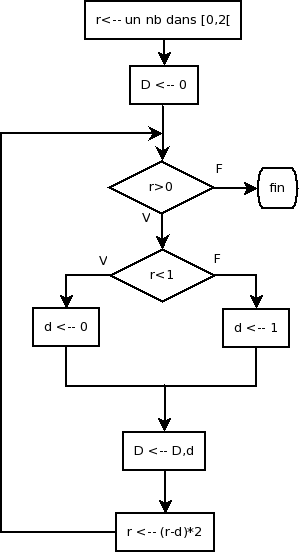
\includegraphics[width=7cm]{Ebincos_1.png}
 \caption{Développement binaire}
 \label{fig:Ebincos_1}
\end{figure}
\begin{enumerate}
 \item En discutant suivant $a$ dans $[0,2[$, préciser $d_0$ et $r_0$.
 \item Soit $n$ un entier donné. En complétant le diagramme de la figure \ref{fig:Ebincos_1}, former un algorithme permettant d'afficher 
\begin{displaymath}
 0,d_0,d_1,\cdots,d_n \text{ et } r_n
\end{displaymath}
lorsque $r_n\neq 0$.
\end{enumerate}


\subsection*{PARTIE II : itération d'une fonction}
On définit la fonction $f$ dans $\R$ par :
\begin{displaymath}
 \forall x\in \R: f(x) = 2x^2 - 1
\end{displaymath}
\begin{enumerate}
 \item Déterminer les réels $x$ tels que $f(x)=x$ (points \emph{fixes}).
 \item Former le tableau des variations de $f$ et tracer son graphe en précisant les points d'abscisse $-1$ et $1$.
 \item On définit une suite de réels $\left( v_n\right) _{n\in \N}$ par :
\begin{align*}
  &v_0 \in [-1,1]\\
  &\forall n\in \N : v_{n+1}= f(v_n)
\end{align*}
\begin{enumerate}
 \item Montrer que $v_n\in [-1,1]$ pour tous les naturels $n$.
 \item Soit $\theta=\arccos(v_0)$. Montrer que $v_n = \cos(2^n \theta)$ pour tous les entiers $n$.
\end{enumerate}
\end{enumerate}

\subsection*{Partie III : suite de signes et développement binaire}
Dans cette partie, $a$ est un {\'e}l{\'e}ment de $] 0,2[$ et on utilise les notations  $\left( d_n\right) _{n\in \N}$,  $\left( r_n\right) _{n\in \N}$,  $\left( v_n\right) _{n\in \N}$ des deux premières parties avec
\begin{displaymath}
v_0=\cos \frac{a\pi}{2} 
\end{displaymath}
\begin{enumerate}
\item  Soit $n$ un entier quelconque.
\begin{enumerate}
 \item Montrer qu'il existe $m\in \N$ et $h\in \left[ 0,\frac{1}{2}\right[ $ tels que
\begin{displaymath}
2^{n}a =2m+d_{n}+\frac{1}{2}d_{n+1}+h 
\end{displaymath}
\item En distinguant les quatre cas possibles pour les valeurs de $d_n$ et $d_{n+1}$, exprimer $v_{n+1}$ uniquement avec des valeurs en $h$ de fonctions trigonométriques.
\item Montrer que, pour tout naturel $n$ tel que $r_{n+1}\neq 0$,
\begin{displaymath}
(-1)^{d_n + d_{n+1}}v_{n+1} > 0       
\end{displaymath}
\end{enumerate}
\item  Expliquer comment, à partir de $a$, on peut calculer la suite $(d_{n})_{n\in \N}$ par r{\'e}currence {\`a} l'aide de $(v_{n})_{n\in \N}$. Former un schéma associé à cet algorithme.

\item  En utilisant l'algorithme pr{\'e}c{\'e}dent, calculer le d{\'e}veloppement binaire {\`a} l'ordre $7$ de $\frac{2}{3}$.
\item On suppose que $a$ est rationnel : $a=\frac{p}{q}$ avec $p$ et $q$ naturels vérifiant $0<p<2q$. Montrer, en utilisant l'algorithme de la question 2., que le développement binaire de $a$ est \emph{finalement-périodique} c'est à dire qu'il existe $m$ et $u$ dans $\N$ tels que 
\begin{displaymath}
 \forall n\in \N : n\geq m \Rightarrow d_{n+u} = d_n
\end{displaymath}
\end{enumerate}
